\chapter{Lie theory and Jacobi diagrams}
\label{ch:lie-theory-and-jacobi-diagrams}

The fundamental theorem of Vassiliev invariants states that the bialgebra of Vassiliev invariants can be broken up into nice combinatiorial weight systems. So to understand \(\mathcal{V}\) it suffices to understand \(\mathcal{W}\), or equivalently its dual \(\mathcal{A}\). There is a hint that the structure of \(\mathcal{A}\) may relate to Lie algebras.

\begin{mdframed}
	The hint is that Hopf algebras have a lie algebra as their primitive elements \(\mathcal{P}(H)\). However I clearly am confused here, for the following reason. By the Milnor-Moore theorem, applying this to \(\mathcal{A}\), it should be the symmetric algebra (and therefore the universal enveloping algebra, as it's abelian?) of \(\mathcal{P}(\mathcal{A})\).

	However this clashes with my understanding of the raison d'etre of Hinnich-Vaintrob \cite{cyclic-operads-and-the-algebra-of-chord-diagrams}. According to them, the point of their convoluted construction is to realise \(\mathcal{A}\) as the universal enveloping algebra of some Lie algerba. And a key point is that that's not technically true, hence the need to move to more general tensor categroies.

	Further evidence in \cite{noncommutative-chern-weil-theory-and-the-combinatorics-of-wheeling}: ``The STU relation is a formal analogue of the relation in a Universal Enveloping Algebra which equates a commutator with the corresponding bracket'' (the word formal implying that this isn't literally true).

	Page 141 on \cite{introduction-to-vassiliev-invariants} furthermore says that \cite{cyclic-operads-and-the-algebra-of-chord-diagrams} shows \(\mathcal{A}\) (algebra of Jacobi diagrams on the circle) is isomorphic to the center of the universal enveloping algebra of a Casimir Lie algebra in a certain tensor category. Indeed that's my interpretation of HV, but why do if we already know that \(\mathcal{A}\) is already the center (which in this case equals the whole thing) of \(\mathcal{P}(\mathcal{A})\)?!
\end{mdframed}

\begin{mdframed}
Scaffold of chapter:

	-- That 4T looks like STU/IHX. Hint at Lie algebra relations.

	-- The isomorphism from Chord diagrams to Jacobi diagrams with proof.

	-- Bar-Natan construction: Lie algebra \(\to\) some weight systems. i.e. you get a quotient(?) of \(\mathcal{A}\) from this?

	-- Some examples of this, and some talking about diagrams not detected by Lie algebras (who?), even Lie Superalgebras (Vogel). Perhaps also some dimensions of spaces.

	-- Go through classical Hinnich-Vaintrob.
\end{mdframed}

% TODO: Try to fix(?) and include the below CDM proof of Milnor-Moore
% \begin{theorem}
% 	The bialgebra \(\mathcal{A}\) is canonically isomorphic to the algebra of polynomials in its primitive elements,
% 	\[\mathcal{A} \cong S(\mathcal{P}(\mathcal{A})),\]
% 	where \(S\) denotes the symmetric algebra.
% \end{theorem}
% \begin{proof}
% 	\begin{mdframed}
% 		The proof in \cite{introduction-to-vassiliev-invariants} is readable, but missing crucial details, and containing a typo. Furthermore I cannot find it anywhere else. If there is time, I want to find out if it works and include it. Perhaps compare to the original source.
% 	\end{mdframed}
% \end{proof}

\section{Jacobi diagrams, AS, STU and IHX}

This side of the story reframes the algebra \(\mathcal{A}\) as a separate algebra to make the Lie theory connection more obvious.

\begin{definition}
	A \textbf{unitrivalent diagram} is a unitrivalent graph (with loops and multiple edges allowed) with the following additional data:
	\begin{itemize}
		\item each trivalent vertex has a fixed cyclic order of incident edge-connections,
		\item the set of univalent vertices has a fixed cyclic order.
	\end{itemize}
	The vector space of unitrivalent diagrams is denoted \(\mathcal{T}\).
\end{definition}

When drawing unitrivalent diagrams, we specify the fixed cyclic order of the univalent edges of a unitrivalent diagram by drawing them connected to a circle. In particular all chord diagrams are Jacobi diagrams with only univalent vertices (the chord ends). Further examples of non-chord diagram Jacobi diagrams would be
\[
	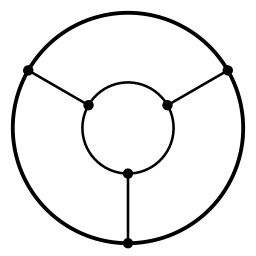
\includegraphics[width=0.13\textwidth, valign=c]{graphics/unitrivalent_diagram_example_1.pdf} \ ,
	\quad
	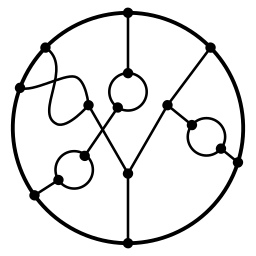
\includegraphics[width=0.13\textwidth, valign=c]{graphics/unitrivalent_diagram_example_2.pdf}
	\in \mathcal{T}.
\]

\begin{definition}
	The \textbf{STU relation} is the relation
		\begin{equation}
			\label{eq:STU}
			\tag{\stu}
			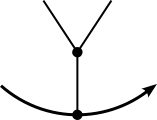
\includegraphics[width=0.10\textwidth, valign=c]{graphics/stu_relation_s.pdf}
			\quad
			=
			\quad
			\includegraphics[width=0.10\textwidth, valign=c]{graphics/stu_relation_t.pdf}
			\quad
			-
			\quad
			\includegraphics[width=0.10\textwidth, valign=c]{graphics/stu_relation_u.pdf}.
		\end{equation}
\end{definition}

As usual, this is not an individual relation but a type of relations, true in any diagrams that are identical except for the subdiagrams being as shown.

Note that the \ref{eq:STU} relations imply the \ref{eq:4T} relations.

\begin{definition}
	The algebra \(\mathcal{J}\) of Jacobi diagrams is the algebra \(\mathcal{T} / \ref{eq:STU}\), with the product \(\connect\) defined the same way as it was for chord diagrams.
\end{definition}

\begin{definitions}
		\item The \textbf{AS relation} (antisymmetry relation) is the relation
			\begin{equation}
				\label{eq:AS}
				\tag{\as}
				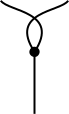
\includegraphics[width=0.05\textwidth, valign=c]{graphics/as_relation_a.pdf}
				\quad
				=
				\quad
				-
				\includegraphics[width=0.05\textwidth, valign=c]{graphics/as_relation_s.pdf}.
			\end{equation}
		\item The \textbf{IHX relation} is the relation
			\begin{equation}
				\label{eq:IHX}
				\tag{\ihx}
				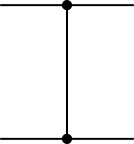
\includegraphics[width=0.10\textwidth, valign=c]{graphics/ihx_relation_i.pdf}
				\quad
				=
				\quad
				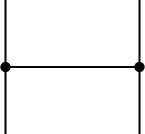
\includegraphics[width=0.10\textwidth, valign=c]{graphics/ihx_relation_h.pdf}
				\quad
				-
				\quad
				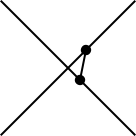
\includegraphics[width=0.10\textwidth, valign=c]{graphics/ihx_relation_x.pdf}.
			\end{equation}
\end{definitions}

\section{Lie algebra weight systems}

\section{Jacobi diagrams as a universal enveloping algebra}
